\chapter{Introduction}\label{introduction}
\section{Problem statement}
With the advance of \emph{deep reinforcement learning} in $2013$, \emph{intelligent agents} have increasingly been able to solve more complex problems \cite{deeprl}. In reinforcement learning (RL), an agent is trained to solve a problem through trial and error, using feedback in the form of rewards. This way it tries to find an optimal \emph{policy}: a mapping of a state and its available actions to a valuation for each action. For \emph{deep} RL, \emph{artificial neural networks} are used to train such an agent. The usage of increasingly complex problem settings comes with more complex environments for an agent to work in; observations representing the current state of the environment are becoming dimensionally higher.
	
This means that the \emph{state-space} of the environment, the number of possible states the environment can be in, is increasing. In general, the larger the state-space, the more difficult and time intensive the training of the agent will be, and thus the more computing cost is needed. This is due to several reasons. Firstly, with a larger state-space, the agent will need to explore more states before having explored the entire state-space. This leads to having to gather larger datasets of state observations which can be impractical \cite{AE_2019}.

Secondly, for deep RL, the agent uses artificial neural networks. These networks need to be of a size proportional to the state-space to be able to accurately approximate an optimal policy; otherwise it could lead to under-fitting or over-fitting \cite{rlfitting}. Generally, the larger the state-space, the larger such a network needs to be. This means the network will contain more trainable parameters, leading to more computation for its training and its usage \cite{AE_2019}.

Lastly, higher dimensional states may include more irrelevant information and noise. This can lead to longer training times and even to agents not being able to find optimal policies \cite{AE_2016}.

\section{Research questions}
A way for dealing with large state-spaces is needed for RL to be scalable. One way to deal with this, is by lowering the state-space of a specific problem, whilst retaining enough state information for the agent to find an optimal policy. This is known as \emph{state-space dimensionality reduction}. Here, a state observation would be projected to a lower dimensional space; this lower dimensional representation is called the \emph{latent representation}. The main problem with state-space dimensionality reduction, is the loss of possibly essential information, which could lead to RL agents not being able to find an optimal policy. Capturing the dynamics of all states in a lower dimensional space, is also known as \emph{state representation learning} \cite{representation_overview}.

In this thesis, we will examine the effect of using state-space dimensionality reduction on an RL agent, focusing on whether an agent can find optimal policies on a lower dimensional state-space. More specifically, we will look at the effect on a model-free, value based RL agent (as explained in section \ref{pl-rl}). For this, we will use the \emph{double deep-Q-network} (DDQN) learning algorithm (see section \ref{pl-dqn}) \cite{ddqn}. We will project the state observations to a lower dimensional space using three different methods, whose effects on the RL agent we will compare: \emph{principal component analysis}, \emph{autoencoders} and \emph{DeepMDPs} (see sections \ref{pl-pca}, \ref{pl-ae} and \ref{pl-deepmdp} respectively for information about each method). We will apply these methods on two environments that use high dimensional grid-based observations: Starcraft II MoveToBeacon (see \ref{research-env-pysc2}) and OpenAI Atari Pong (see \ref{research-env-pong}) \cite{pysc2}\cite{pong}. We will examine the retainment of the observations' spatial information after state-space dimensionality reduction.

The \textbf{main research question} we will examine is:\newline

\noindent \textit{What is the effect of state-space dimensionality reduction on model-free value-based reinforcement learning in an environment using spatial grid-based observations, by using Principal Component Analysis, autoencoders or DeepMDPs}? \newline

\noindent To answer this, we will answer the \textbf{research sub-question}:\newline

\noindent \textit{How do the training results of a double deep-Q-network reinforcement learning agent change when using Principal Component Analysis, autoencoders and DeepMDPs for state-space dimensionality reduction in Starcraft II MoveToBeacon and OpenAI Atari Pong}?

\section{Method, results and possible benefits}
We gathered the training results for several RL agents trained in Starcraft II and Pong. The first agent is a baseline agent: a DDQN RL agent using the observations given by the environment. Apart from this, there are four agents using different state-space dimensionality reduction methods. These RL agents train on observations projected to a lower dimensional space. This interaction can be seen in figure \ref{fig:rl_cycle_dimred}. Firstly, the PCA agent uses Principal Component Analysis (PCA) to reduce the dimensionality of the observations. Thus, the observations given by the environment first go through PCA, thereby projected to a lower dimensional space, before being used by the RL agent. The PCA is trained on previously stored observation traces, before being used by the RL agent. This process is shown in figure \ref{fig:rl_training}. There are also two agents using an autoencoder, that work similar to the PCA agent. The first of the two uses a pre-trained autoencoder, again trained on stored observations (again shown in figure \ref{fig:rl_training}). The second autoencoder agent, the online trained autoencoder agent, is trained simultaneously with the RL agent, using the observations received by the agent. Lastly, there is a DeepMDP agent, which is only used in the Starcraft II environment.

In both environments, the PCA agent lost all spatial information, leading to RL agents learning sub-optimal policies. The DeepMDP was also unable to train to an optimal policy in Starcraft II. However, the autoencoder agents were able to learn good policies (nearing an optimal, scripted agent's score at around $80\%$). In the Starcraft II environment, the pre-trained autoencoder agent learned a better, more stable policy in less episodes than the baseline agent (having on average a $10\%$ improvement using $400$ instead of $600$ episode converge). The online trained autoencoder agent had training results similar to the baseline agent, yet slightly more inconsistent, needing $500$ episodes to converge. Similar results were found for the second environment, Pong. However, the pre-trained autoencoder agent learned a slightly worse policy than the baseline agent (a $20\%$ decrease). This resulted from the agent needing more precise spatial information (capturing the original state dynamics better) than in the Starcraft II environment; the consequences of grouping together multiple similar states (e.g. two states where the location of a single object differs by one grid-cell) into a single latent state are greater in Pong than in Starcraft II. The online trained autoencoder agent again converged to a policy similar to the pre-trained autoencoder agent, but needing slightly more episodes to converge. In the Pong environment we also show that RL agents training on less accurate latent representations, meaning they capture the original state dynamics less, result in worse policies. The (possible) dependence of an RL agent on the retainment of spatial information for finding an optimal policy, shows a limit with regards to the usage of an autoencoder agent.

Several benefits may arise from training agents on lower state-spaces. Though we will mention these benefits now here, the extend of these benefits is not examined in this thesis and is left for future research.

Firstly, RL agents training in a lowered state-space might need less training time and less observation data, and therefore less computational cost for training and using its neural network. 

Secondly, in very complex, large scaled environments, a normal RL agent might not be able to explore the entire state-space in a feasible amount of time, possibly resulting in a sub-optimal policy; here, state-space dimensionality reduction could to result in a better policy. 

Thirdly, depending on the dimensionality reduction method, we could reuse the dimensionality reduction component in different RL agents solving different problems in the same environment. Thus, we would only have to train a dimensionality reduction component once, then being able to train different agents on the same latent representation. This possibility though depends on two things. It would need to be a dimensionality reduction method that is trainable separately from the RL agent. This is the case for only two of the three methods we consider in our research: PCA and autoencoders. Secondly, the latent representation would have to be problem-agnostic: it would have to be a good representation of the entire state-space, without losing information essential to any of the RL problems being used in this environment.


\begin{figure}[h]
	\centering
	\begin{subfigure}[b]{0.20 \textwidth}
		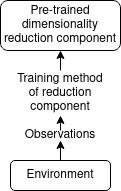
\includegraphics[width=\linewidth]{rl_dimred_training}
		\caption{High level overview of training a state-space dimensionality reduction component; used for training the PCA and autoencoder components.}
		\label{fig:rl_training}
	\end{subfigure}\hfill
	\begin{subfigure}[b]{0.50\textwidth}
		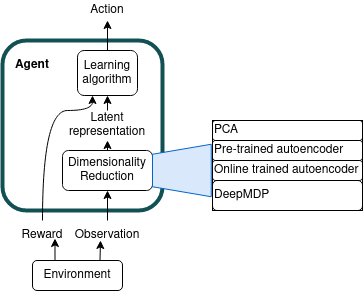
\includegraphics[width=\textwidth]{rl_cycle_dim_red_intro}
    		\caption{Overview of the general architecture of an RL agent using a state-space dimensionality reduction method, including the reduction methods used in our experiments. The learning algorithm used is DDQN.}
    		\label{fig:rl_cycle_dimred}
	\end{subfigure}
	\caption{Overview of the process of training the state-space dimensionality reduction components for PCA and autoencoders, and their usage in an RL agent}.
\end{figure}
	

\section{Paper structure}
We will start by discussing related work in section \ref{relatedwork}, before giving preliminary information in section \ref{preliminaries}. In this preliminary section we will first give an overview of reinforcement learning principles in section \ref{pl-rl}. This will include an explanation of artificial neural networks and the RL learning algorithm DDQN, which we use for our agents. After this, we will discuss state-space dimensionality reduction in section \ref{pl-dimensionality}, which will include an examination of the three methods used in our research: PCA, autoencoders and DeepMDPs.

After the preliminaries, we will show our methodology in section \ref{research-method}. Here we will give a general overview of the different RL agents that we will use for our experiments. Then we will give information about the environments used and the specific agent setups per environment. 

After having explained the experiment setups, we will give the results of our experiments in section \ref{research-results}. We will show and discuss the results per environment, before discussing the results of both environments as a whole.

Next, we will give our conclusions and suggestions for future research in section \ref{conclusions}. Lastly, the appendices in section \ref{appendix} will contain more details on the specific agent architectures per environment, including hyperparameter settings.

Our code repository can be found at: \url{https://github.com/Niels-vv/Safe-RL-With-DR.git}.